% ===========================================================
%  Лекция 11. Задача о максимальном потоке в сети.
%             Метод проталкивания предпотока
% ===========================================================

\chapter{Лекция 11. Задача о максимальном потоке в сети}

\subsection*{Метод (алгоритм) проталкивания предпотока}

Идея метода: в отличие от Форда--Фалкерсона, который наращивает поток
целыми путями $S \to F$, здесь мы разрешаем вершинам временно
\emph{накапливать} лишний втекающий поток (избыток) и затем
<<проталкивать>> его дальше --- как вода, стекающая по каскаду
резервуаров разной высоты.

\begin{defn}{Предпоток}{predpotok}
Пусть $G$~--- сеть, $\sigma$~--- пропускная способность рёбер.

\textbf{Предпоток}~--- это функция $\tilde{f}\colon V \times V \to \mathbb{R}$, удовлетворяющая условиям:
\begin{enumerate}
  \item \textbf{Ограниченность:} $\forall\, e = uv\colon -\sigma(e) \le \tilde{f}(u,v) \le \sigma(e)$;
  \item \textbf{Кососимметричность:} $\forall\, u,v \in V\colon \tilde{f}(u,v) = -\tilde{f}(v,u)$;
  \item $\forall\, \nexists\, e = uv,\; e = vu \;\Rightarrow\; \tilde{f}(u,v) = 0$.
\end{enumerate}
В отличие от потока, условие балансировки \emph{не требуется}: в вершину
может втекать больше, чем вытекает.
\end{defn}

\begin{defn}{Эксцесс вершины}{excess}
\textbf{Эксцесс вершины} $\forall\, v \in V$:
\[
  \varepsilon(v) := \sum_{w \in P(v)} \tilde{f}(\overline{wv}) - \sum_{u \in \mathrm{Ch}(v)} \tilde{f}(\overline{vu}),
\]
где $P(v)$~--- родители, $\mathrm{Ch}(v)$~--- дети
(т.\,е.\ эксцесс --- это <<втекло минус вытекло>>).
\end{defn}

\textbf{NB.} Если $\forall\, v \in V \setminus \{S, F\}\colon \varepsilon(v) = 0$, то $\tilde{f}$~--- поток.

\begin{defn}{Высота вершины}{height}
\textbf{Высота вершины}~--- это функция $h\colon V \to \mathbb{N}_0$.
Инициализируется как $h(S) = |V|$, $h(v) = 0$ для остальных, и в
процессе работы только растёт. Проталкивать избыток разрешается
только <<вниз>>: из вершины $v$ в вершину $u$ с $h(u) = h(v) - 1$.
\end{defn}

\begin{algo}{Метод проталкивания предпотока (Push-Relabel)}{push-relabel}

\textbf{Инициализация:}
\begin{enumerate}
  \item $h(S) := |V|$; \quad $\forall\, u \in V \setminus \{S\}\colon h(u) := 0$.
  \item $\tilde{f}_{\text{start}}$: $\forall\, v \in \mathrm{Ch}(S)\colon \tilde{f}(S, v) := \sigma(\overline{Sv})$, \quad $\tilde{f}(v, S) := -\sigma(\overline{Sv})$; \\
        $\forall\, u, \hat{v} \in V \setminus \{S\}\colon \tilde{f}(u,v) := 0$
        \quad (рёбра из истока насыщаются полностью).
\end{enumerate}

\textbf{Основной цикл:} Пока $\exists\, v \in V \setminus \{S, F\}$ т.\,ч.\ $\varepsilon(v) > 0$ (\emph{активная} вершина):

\medskip
\textbf{Push (проталкивание):}
если $\exists\, u \in \mathrm{Ch}(v)$ (в остаточной сети) т.\,ч.\ $h(u) < h(v)$:
\[
  \delta_{\text{new}} := \min\bigl\{\varepsilon(v),\; \tilde{\sigma}(\overline{vu})\bigr\},
\]
\[
  \tilde{f}_{\text{new}}(v,u) := \tilde{f}_{\text{old}}(v,u) + \delta_{\text{new}}, \qquad
  \tilde{f}_{\text{new}}(u,v) := -\tilde{f}_{\text{new}}(v,u),
\]
\[
  \tilde{\sigma}_{\text{new}}(v,u) := \tilde{\sigma}_{\text{old}}(v,u) - \delta_{\text{new}}, \qquad
  \tilde{\sigma}_{\text{new}}(u,v) := \tilde{\sigma}_{\text{old}}(u,v) + \delta_{\text{new}}.
\]

Здесь $\tilde{\sigma}(u,v) + \tilde{\sigma}(v,u) = \sigma(v,u)$ для $vu = e$
(остаточные пропускные способности, как в алгоритме Форда--Фалкерсона;
проталкивание по обратному ребру означает \emph{возврат} ранее
протолкнутого потока).

\medskip
\textbf{Lift (подъём):}
если $\nexists\, u \in \mathrm{Ch}(v)$ т.\,ч.\ $h(u) < h(v)$, то
\[
  h(v) := \min_{u \in \mathrm{Ch}(v)} h(u) + 1
\]
(минимум --- по соседям в остаточной сети; после подъёма проталкивание
из $v$ снова возможно).

\medskip
\textbf{Выход:} когда активных вершин не осталось, предпоток стал
потоком (все внутренние эксцессы равны нулю), и этот поток ---
максимальный; $|f| = \varepsilon(F)$.

\medskip
\noindent\textbf{Пример.} Сеть $S, A, B, C, D, F$ с пропускными
способностями (та же топология, что в лекциях 9--10):

\grfig[0.55]{figures/p25-example-1.pdf}{Сеть Push-Relabel: $S,A,B,C,D,F$, $\sigma$ на рёбрах}

\medskip
Протокол работы (каждая строка --- одна операция; $\delta$ --- объём
проталкивания):

\begin{center}
\small
\begin{tabular}{c|l|c|l}
№ & операция & $\delta$ & комментарий \\ \hline
0 & инициализация & --- & $S{\to}A$, $S{\to}B$ насыщены: $\varepsilon(A){=}3$, $\varepsilon(B){=}2$ \\
1 & lift $A$: $h(A){:=}1$ & --- & соседи $A$ имеют $h = 0$, проталкивать некуда \\
2 & push $A \to C$ & 3 & $h(C) = 0 < 1$; $\varepsilon(A){=}0$, $\varepsilon(C){=}3$ \\
3 & lift $B$: $h(B){:=}1$ & --- & \\
4 & push $B \to D$ & 2 & $\varepsilon(B){=}0$, $\varepsilon(D){=}2$ \\
5 & lift $C$: $h(C){:=}1$ & --- & \\
6 & push $C \to F$ & 2 & ребро $C{\to}F$ насыщено; $\varepsilon(C){=}1$ \\
7 & lift $C$: $h(C){:=}2$ & --- & вниз идти некуда: остаточный сосед --- только $A$ ($h{=}1$) \\
8 & push $C \to A$ & 1 & \emph{возврат} по обратному ребру: $A{\to}C$ теперь $2/3$; $\varepsilon(A){=}1$ \\
9 & lift $A$: $h(A){:=}2$ & --- & остаточные соседи: $C\,(h{=}2)$, $B\,(h{=}1)$, $S\,(h{=}6)$ \\
10 & push $A \to B$ & 1 & $h(B) = 1 < 2$; $\varepsilon(B){=}1$ \\
11 & push $B \to D$ & 1 & $\varepsilon(D){=}3$ \\
12 & lift $D$: $h(D){:=}1$ & --- & сосед $F$ имеет $h = 0$ \\
13 & push $D \to F$ & 3 & $\varepsilon(D){=}0$; активных вершин нет --- стоп \\
\end{tabular}
\end{center}

\medskip
\textbf{Итог:} $|f| = \varepsilon(F) = 2 + 3 = 5$; поток по рёбрам:
$S{\to}A = 3$, $S{\to}B = 2$, $A{\to}C = 2$, $A{\to}B = 1$,
$B{\to}D = 3$, $C{\to}F = 2$, $D{\to}F = 3$, $D{\to}C = 0$ ---
условие балансировки выполнено во всех внутренних вершинах.

\medskip
\noindent\textbf{Работа алгоритма по шагам.} Подпись ребра ---
$\tilde f/\sigma$; под каждой вершиной --- её $h$ и $\varepsilon$.
Активная вершина операции --- оранжевая, поднимаемая --- синяя,
ребро проталкивания --- оранжевое, рёбра с положительным потоком ---
зелёные.

\begin{center}\begin{tabular}{cc}
\shortstack{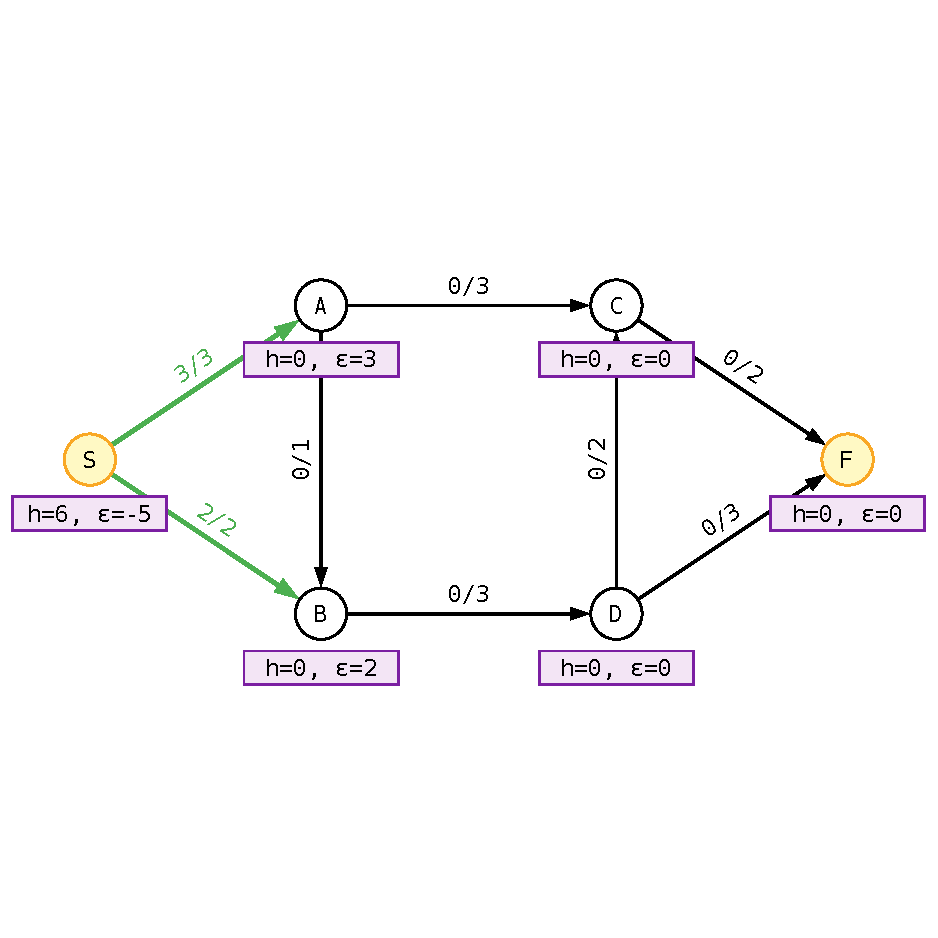
\includegraphics[width=0.46\textwidth]{python/lec11/push_relabel/pr-0.pdf}\\[2pt]{\scriptsize Шаг 0. Инициализация: рёбра из $S$ насыщены}} &
\shortstack{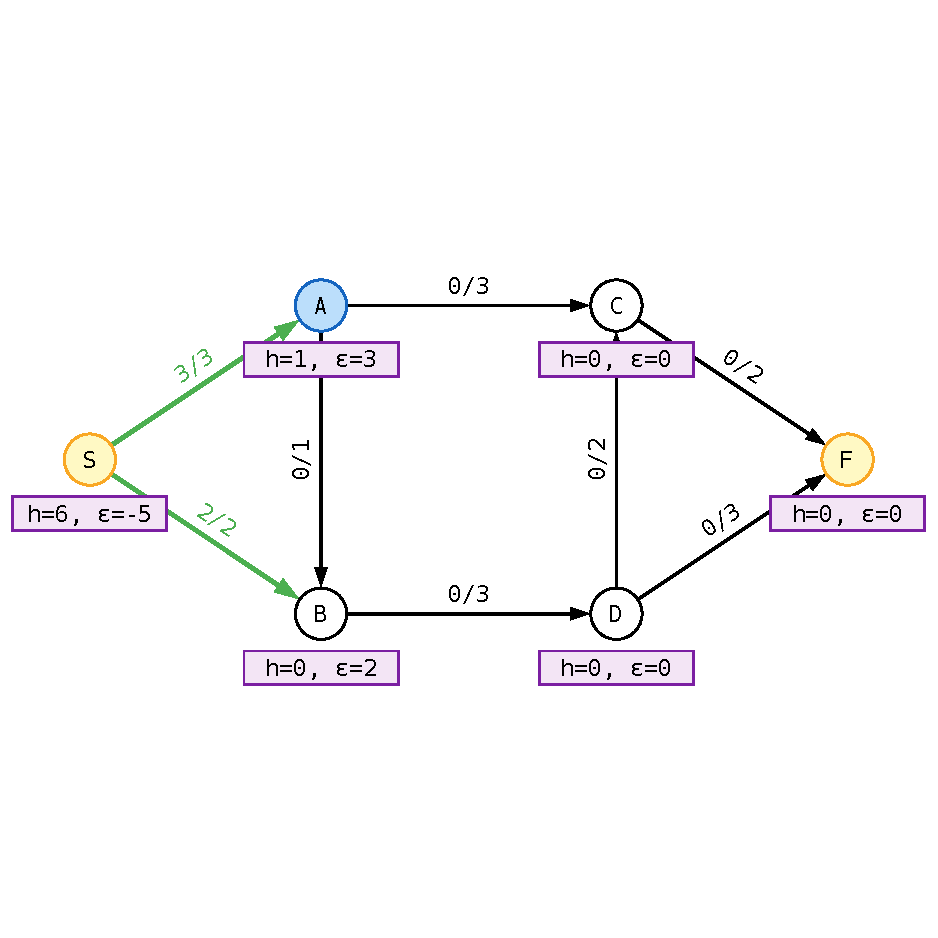
\includegraphics[width=0.46\textwidth]{python/lec11/push_relabel/pr-1.pdf}\\[2pt]{\scriptsize Шаг 1. Lift $A$: $h(A) := 1$}} \\
\end{tabular}\end{center}
\begin{center}\begin{tabular}{cc}
\shortstack{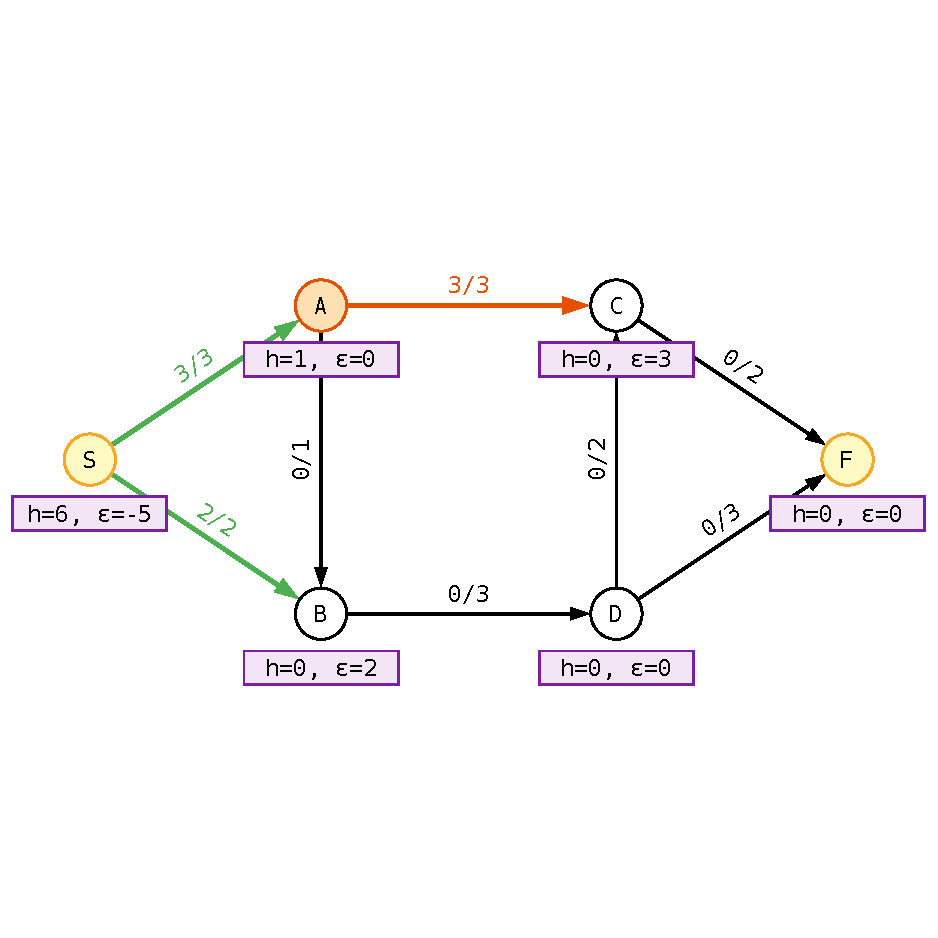
\includegraphics[width=0.46\textwidth]{python/lec11/push_relabel/pr-2.pdf}\\[2pt]{\scriptsize Шаг 2. Push $A \to C$, $\delta = 3$}} &
\shortstack{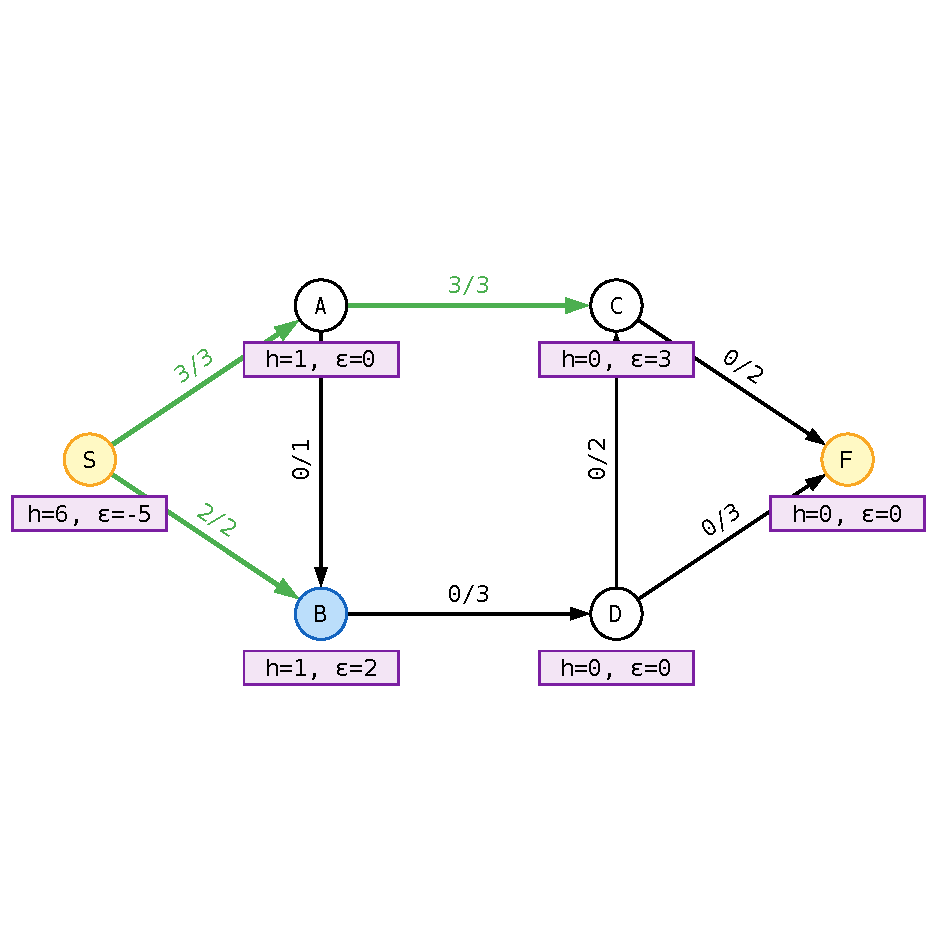
\includegraphics[width=0.46\textwidth]{python/lec11/push_relabel/pr-3.pdf}\\[2pt]{\scriptsize Шаг 3. Lift $B$: $h(B) := 1$}} \\
\end{tabular}\end{center}
\begin{center}\begin{tabular}{cc}
\shortstack{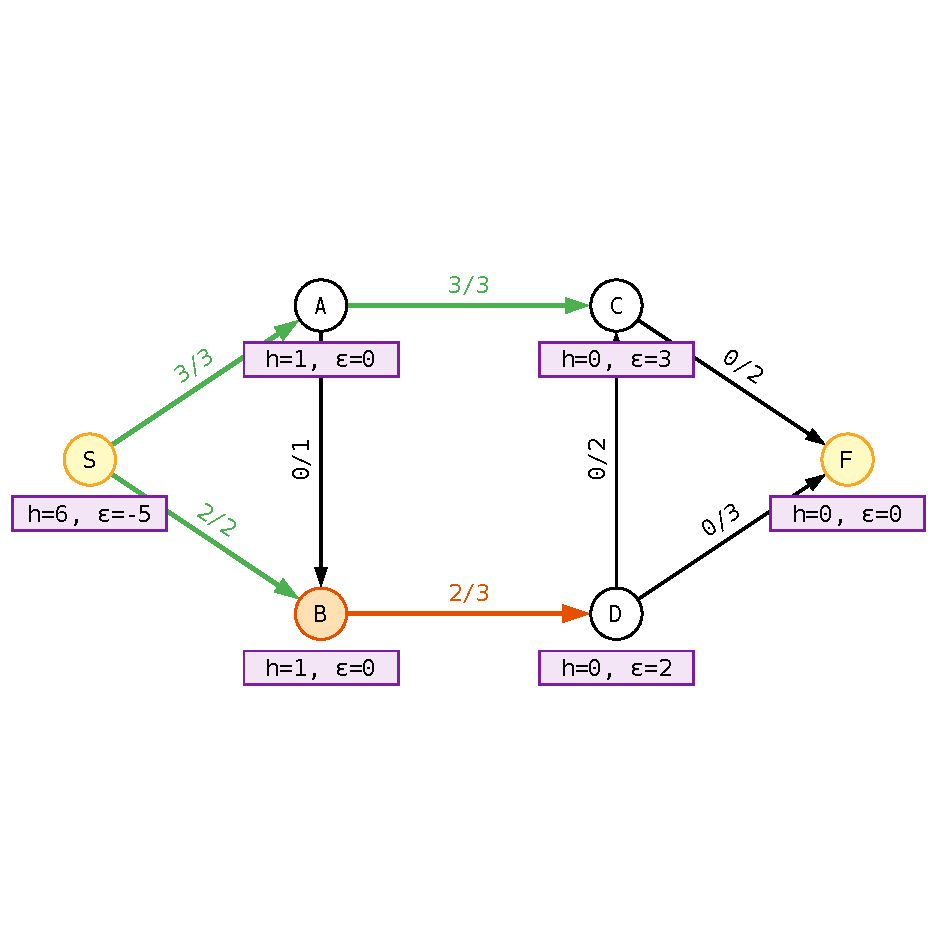
\includegraphics[width=0.46\textwidth]{python/lec11/push_relabel/pr-4.pdf}\\[2pt]{\scriptsize Шаг 4. Push $B \to D$, $\delta = 2$}} &
\shortstack{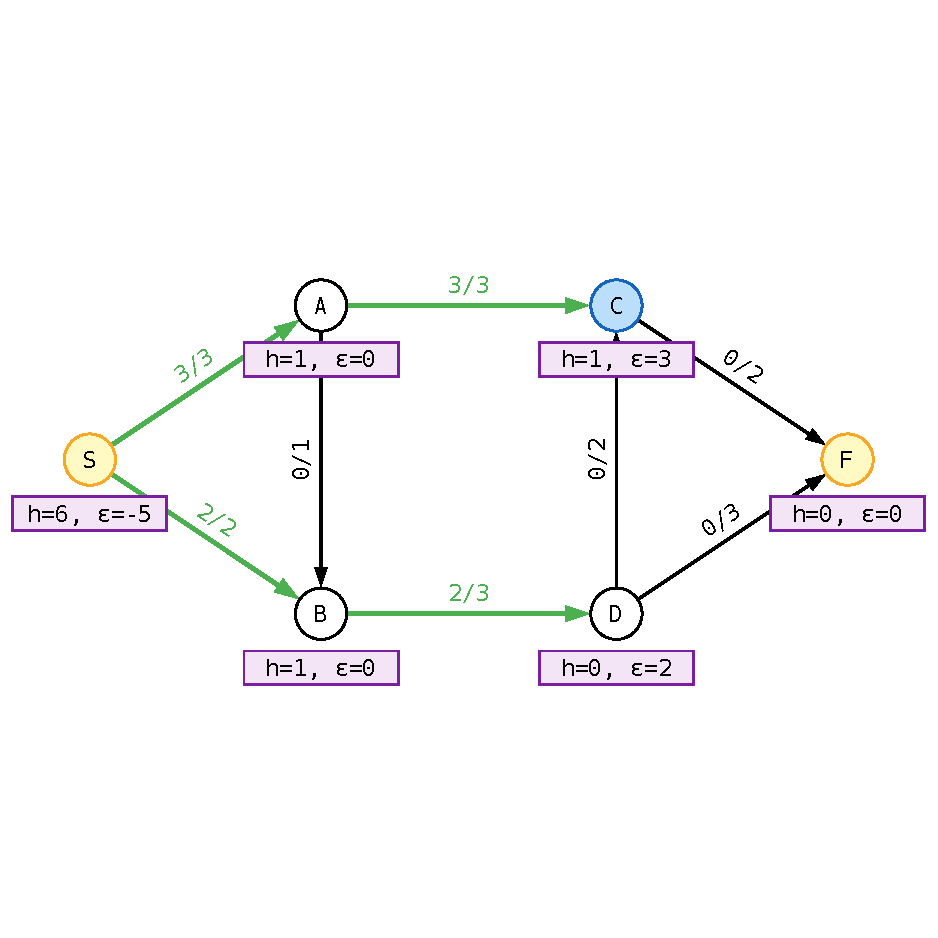
\includegraphics[width=0.46\textwidth]{python/lec11/push_relabel/pr-5.pdf}\\[2pt]{\scriptsize Шаг 5. Lift $C$: $h(C) := 1$}} \\
\end{tabular}\end{center}
\begin{center}\begin{tabular}{cc}
\shortstack{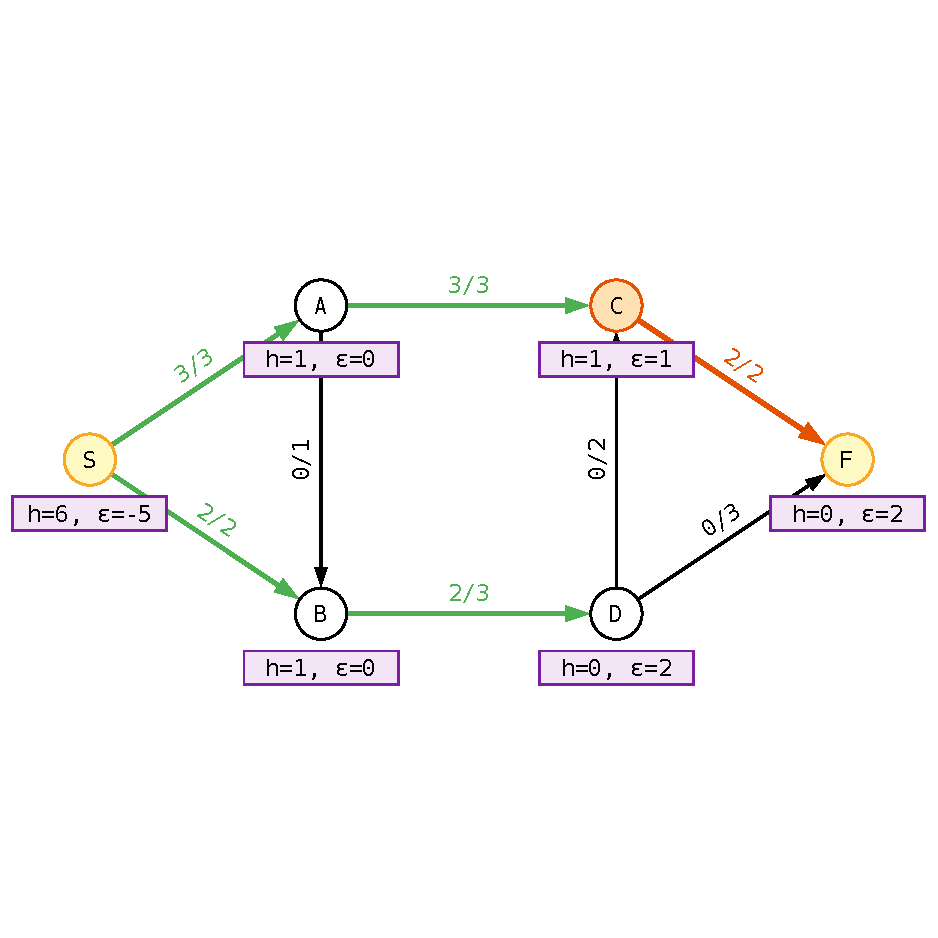
\includegraphics[width=0.46\textwidth]{python/lec11/push_relabel/pr-6.pdf}\\[2pt]{\scriptsize Шаг 6. Push $C \to F$, $\delta = 2$: ребро насыщено}} &
\shortstack{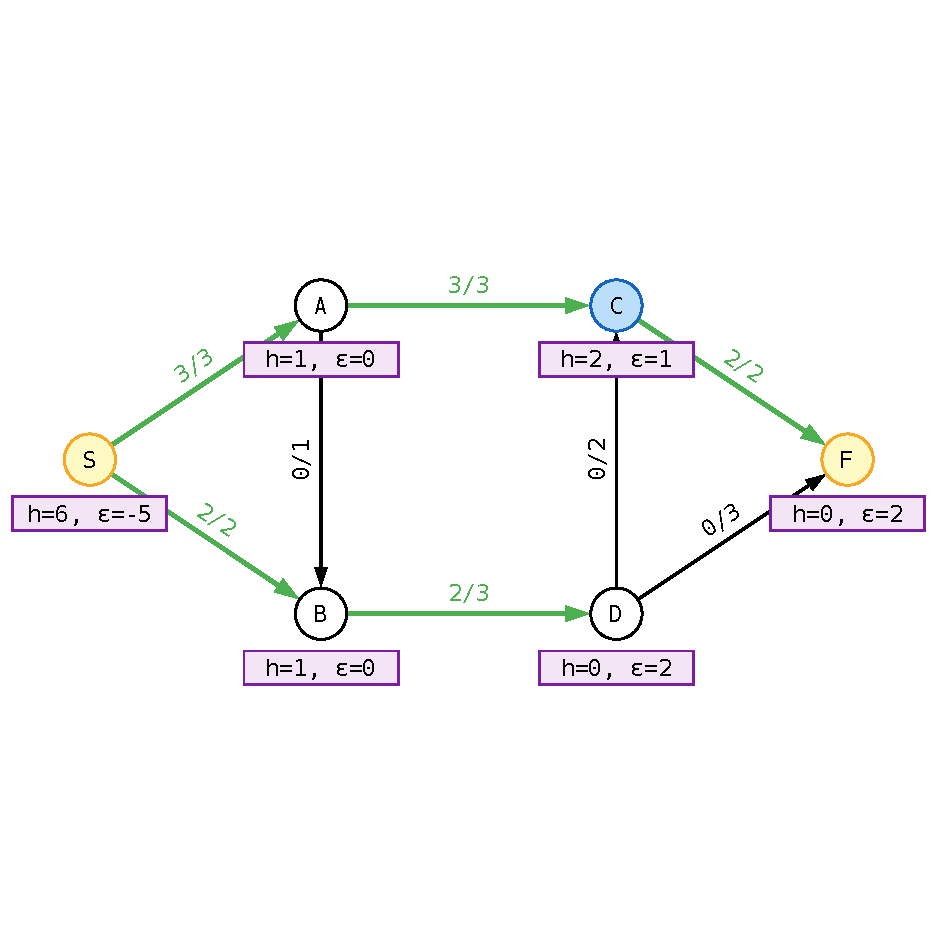
\includegraphics[width=0.46\textwidth]{python/lec11/push_relabel/pr-7.pdf}\\[2pt]{\scriptsize Шаг 7. Lift $C$: $h(C) := 2$ (выше $A$)}} \\
\end{tabular}\end{center}
\begin{center}\begin{tabular}{cc}
\shortstack{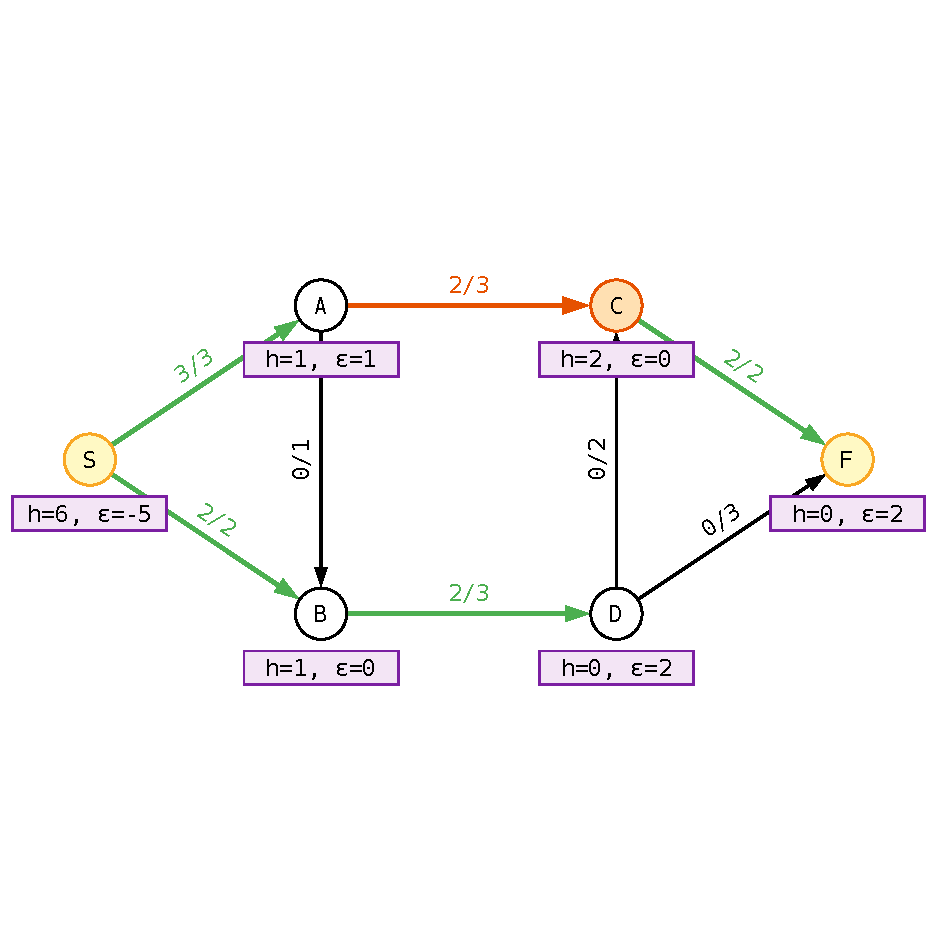
\includegraphics[width=0.46\textwidth]{python/lec11/push_relabel/pr-8.pdf}\\[2pt]{\scriptsize Шаг 8. Push $C \to A$, $\delta = 1$: возврат, $A{\to}C$ стало $2/3$}} &
\shortstack{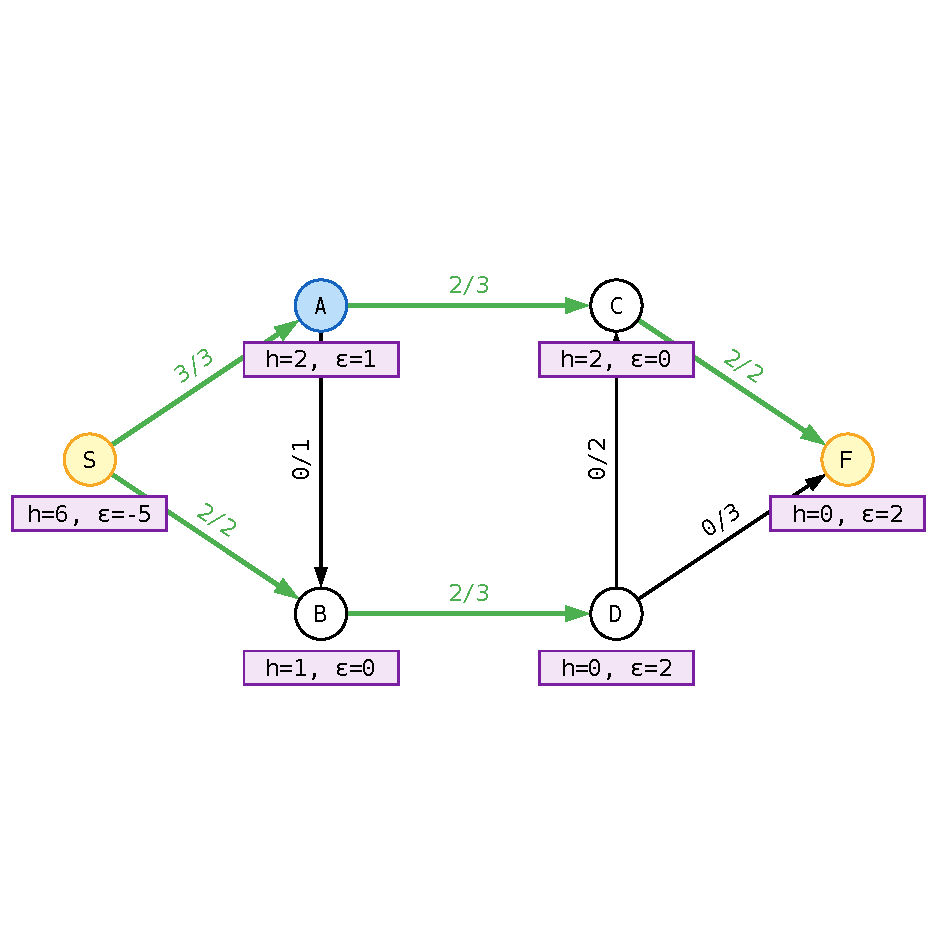
\includegraphics[width=0.46\textwidth]{python/lec11/push_relabel/pr-9.pdf}\\[2pt]{\scriptsize Шаг 9. Lift $A$: $h(A) := 2$}} \\
\end{tabular}\end{center}
\begin{center}\begin{tabular}{cc}
\shortstack{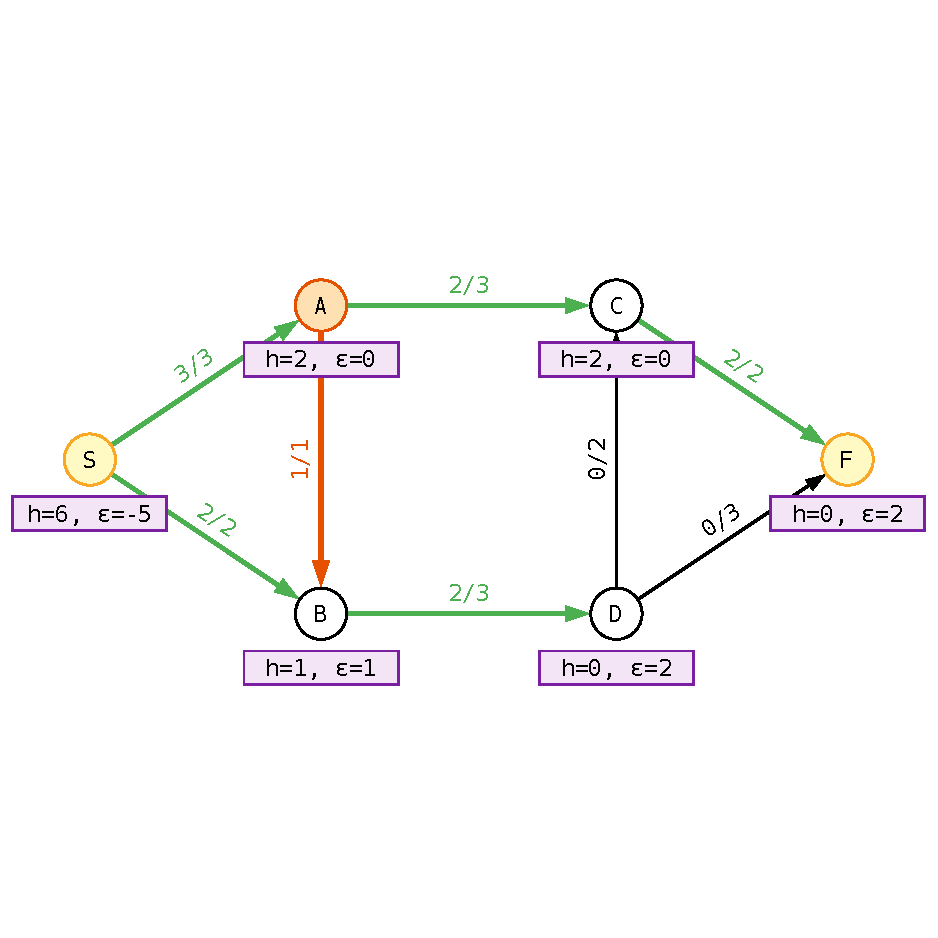
\includegraphics[width=0.46\textwidth]{python/lec11/push_relabel/pr-10.pdf}\\[2pt]{\scriptsize Шаг 10. Push $A \to B$, $\delta = 1$}} &
\shortstack{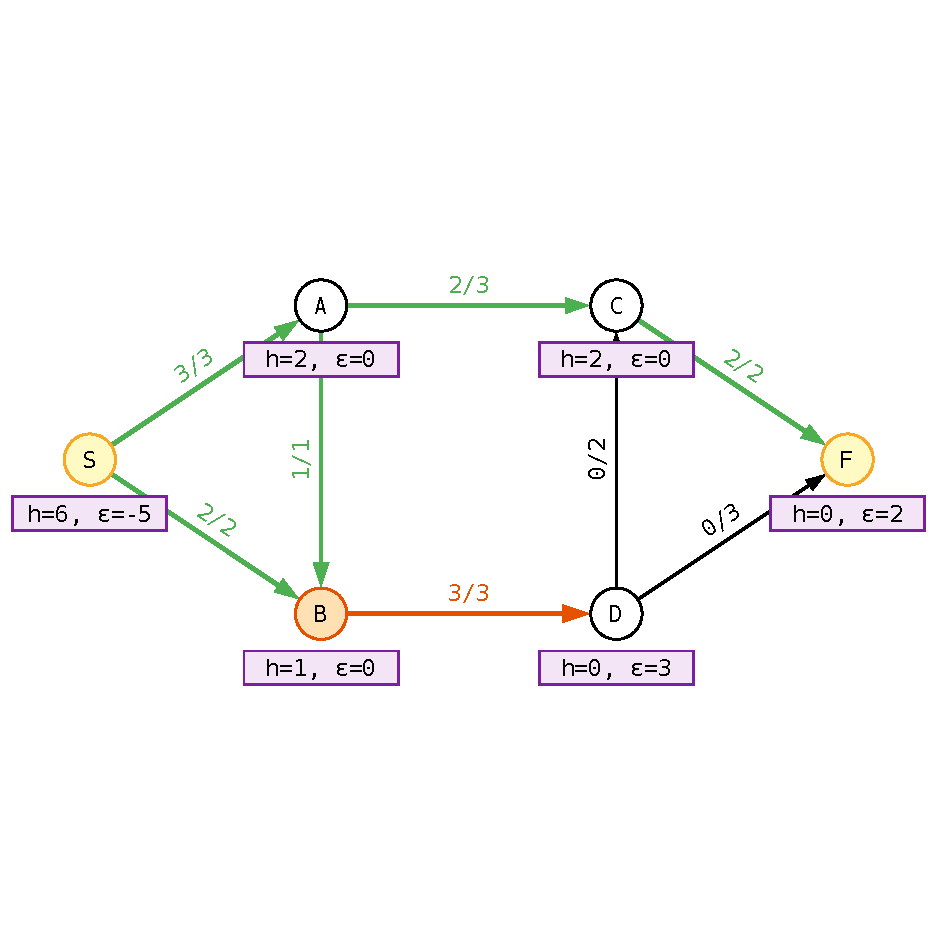
\includegraphics[width=0.46\textwidth]{python/lec11/push_relabel/pr-11.pdf}\\[2pt]{\scriptsize Шаг 11. Push $B \to D$, $\delta = 1$}} \\
\end{tabular}\end{center}
\begin{center}\begin{tabular}{cc}
\shortstack{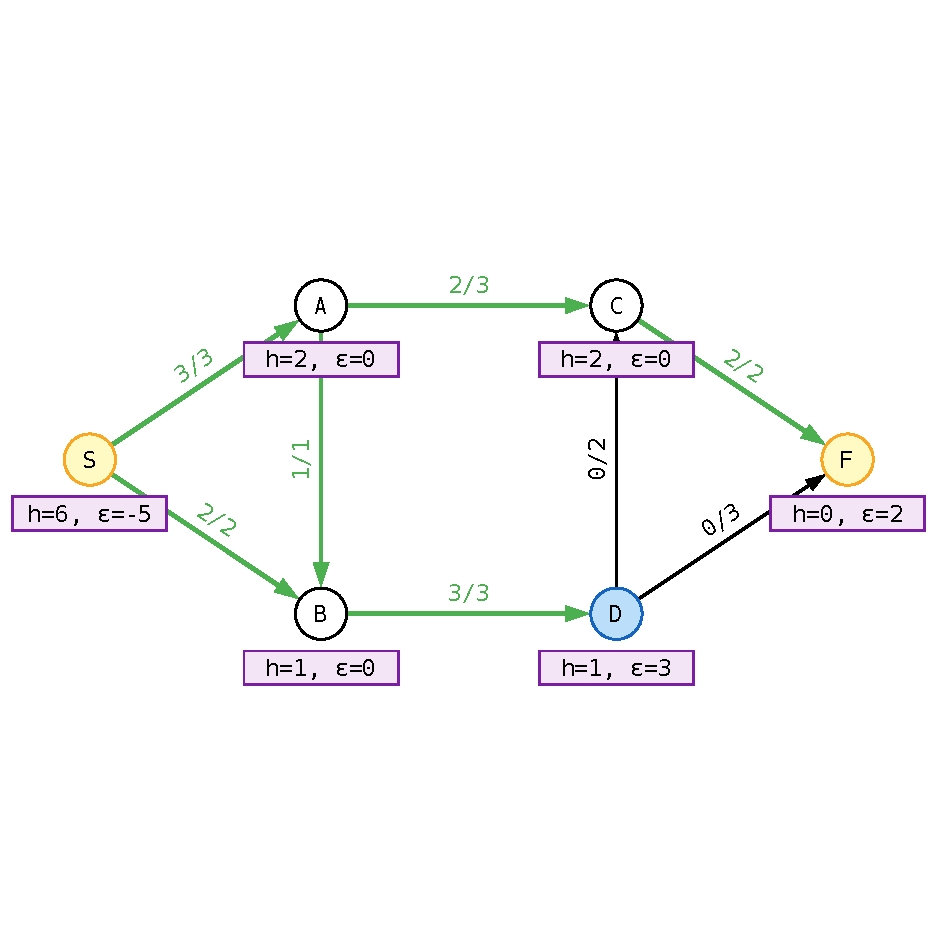
\includegraphics[width=0.46\textwidth]{python/lec11/push_relabel/pr-12.pdf}\\[2pt]{\scriptsize Шаг 12. Lift $D$: $h(D) := 1$}} &
\shortstack{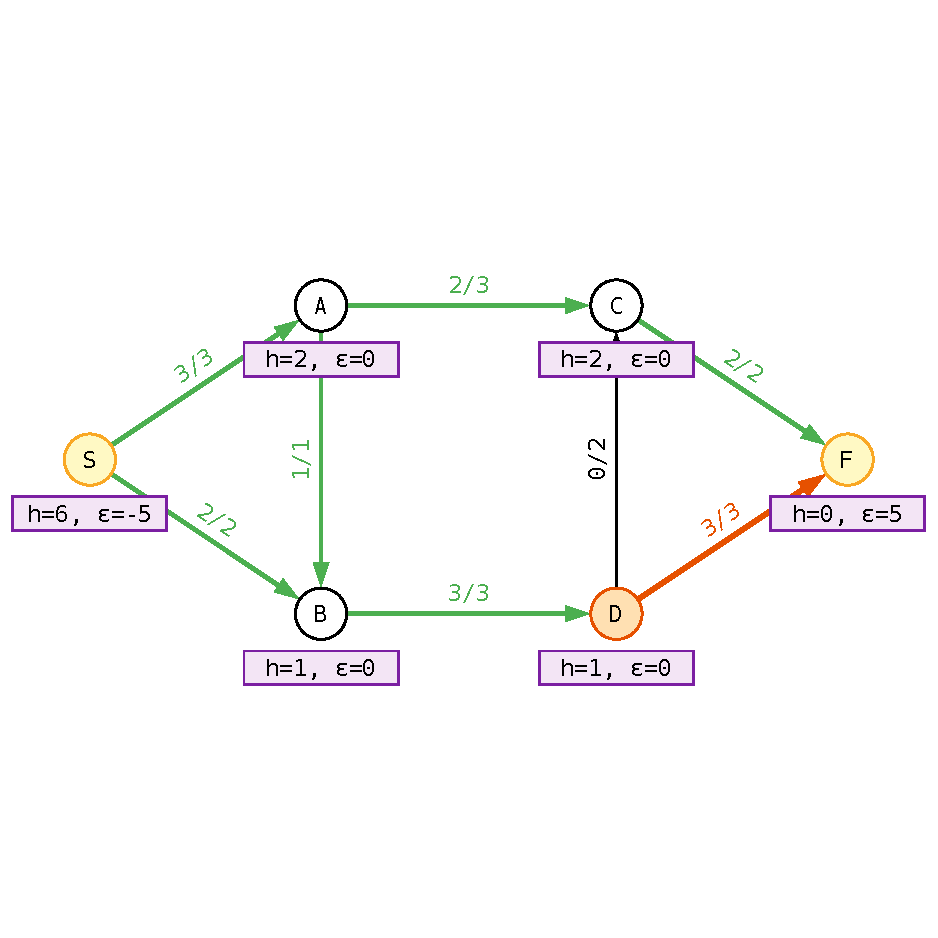
\includegraphics[width=0.46\textwidth]{python/lec11/push_relabel/pr-13.pdf}\\[2pt]{\scriptsize Шаг 13. Push $D \to F$, $\delta = 3$: $|f| = 5$, конец}} \\
\end{tabular}\end{center}
\end{algo}

\medskip
\textbf{Замечание (сумма эксцессов).} В любой момент работы
$\sum_{v \in V} \varepsilon(v) = 0$: каждая единица предпотока на ребре
$uv$ входит в $\varepsilon(v)$ со знаком <<плюс>> и в $\varepsilon(u)$
со знаком <<минус>>, поэтому при суммировании всё сокращается.
В частности, в конце работы $\varepsilon(F) = -\varepsilon(S) = |f|$.

% ===========================================================
%  Хроматика (раскраска графов)
% ===========================================================

\subsection*{Хроматика (раскраска графов)}

\textbf{NB.} Пока рассматриваем \emph{вершинные} раскраски.

\begin{defn}{Правильная раскраска графа}{proper-coloring}
Раскраска графа называется \textbf{правильной}, если любые две смежные вершины окрашены в разные цвета.
\end{defn}

\begin{defn}{Хроматическое число}{chromatic-number}
\textbf{Хроматическое число графа} $\chi(G)$~--- минимальное число цветов, в которые можно правильно раскрасить граф $G$.
\end{defn}

\textbf{Примеры:}
\begin{enumerate}
  \item $|E| = 0 \Rightarrow \chi(G) = 1$: изолированные вершины можно
        красить одним цветом --- конфликтовать нечему.
  \item $|E| > 0 \Rightarrow \chi(G) \geq 2$: у любого ребра концы
        обязаны различаться.
  \item У любого двудольного графа (с рёбрами) $\chi(G) = 2$: красим
        долю $V_1$ первым цветом, долю $V_2$ --- вторым; все рёбра идут
        между долями, конфликтов нет.
  \item $\chi(K_n) = n$: все вершины попарно смежны, поэтому все цвета
        обязаны быть различны (рис.~ниже: $K_4$, $\chi = 4$).
  \item $\chi(C_{2n+1}) = 3$: двух цветов не хватает (нечётный цикл не
        двудолен --- лекция 9), а три цвета есть: чередуем $1, 2$ по
        циклу, последней вершине даём цвет $3$ (рис.~ниже: $C_5$).
        Для чётных циклов $\chi(C_{2n}) = 2$.
\end{enumerate}

\grfig[0.4]{figures/p25-example-2.pdf}{Хром. число: $K_4$, $\chi = 4$ --- все цвета различны}
\grfig[0.4]{figures/p25-example-3.pdf}{Хром. число: $C_5$, $\chi = 3$ --- чередование $1,2$ и третий цвет}

\begin{defn}{Клика}{clique}
\textbf{Клика}~--- максимальный полный подграф графа $G$.
\end{defn}

\begin{lemma}{О клике}{clique-chromatic}
Если $K_n$~--- наибольшая клика в $G$, то $\chi(G) \geq n$.
\end{lemma}

\begin{proof}
Любая правильная раскраска $G$ является правильной и на подграфе $K_n$.
Но в $K_n$ все $n$ вершин попарно смежны, поэтому уже им требуется $n$
различных цветов: $\chi(G) \ge \chi(K_n) = n$.
\end{proof}
